\chapter{Multilevel Stochastic Fairness CoDel}
\label{chap02}

\begin{figure}
	\centering
	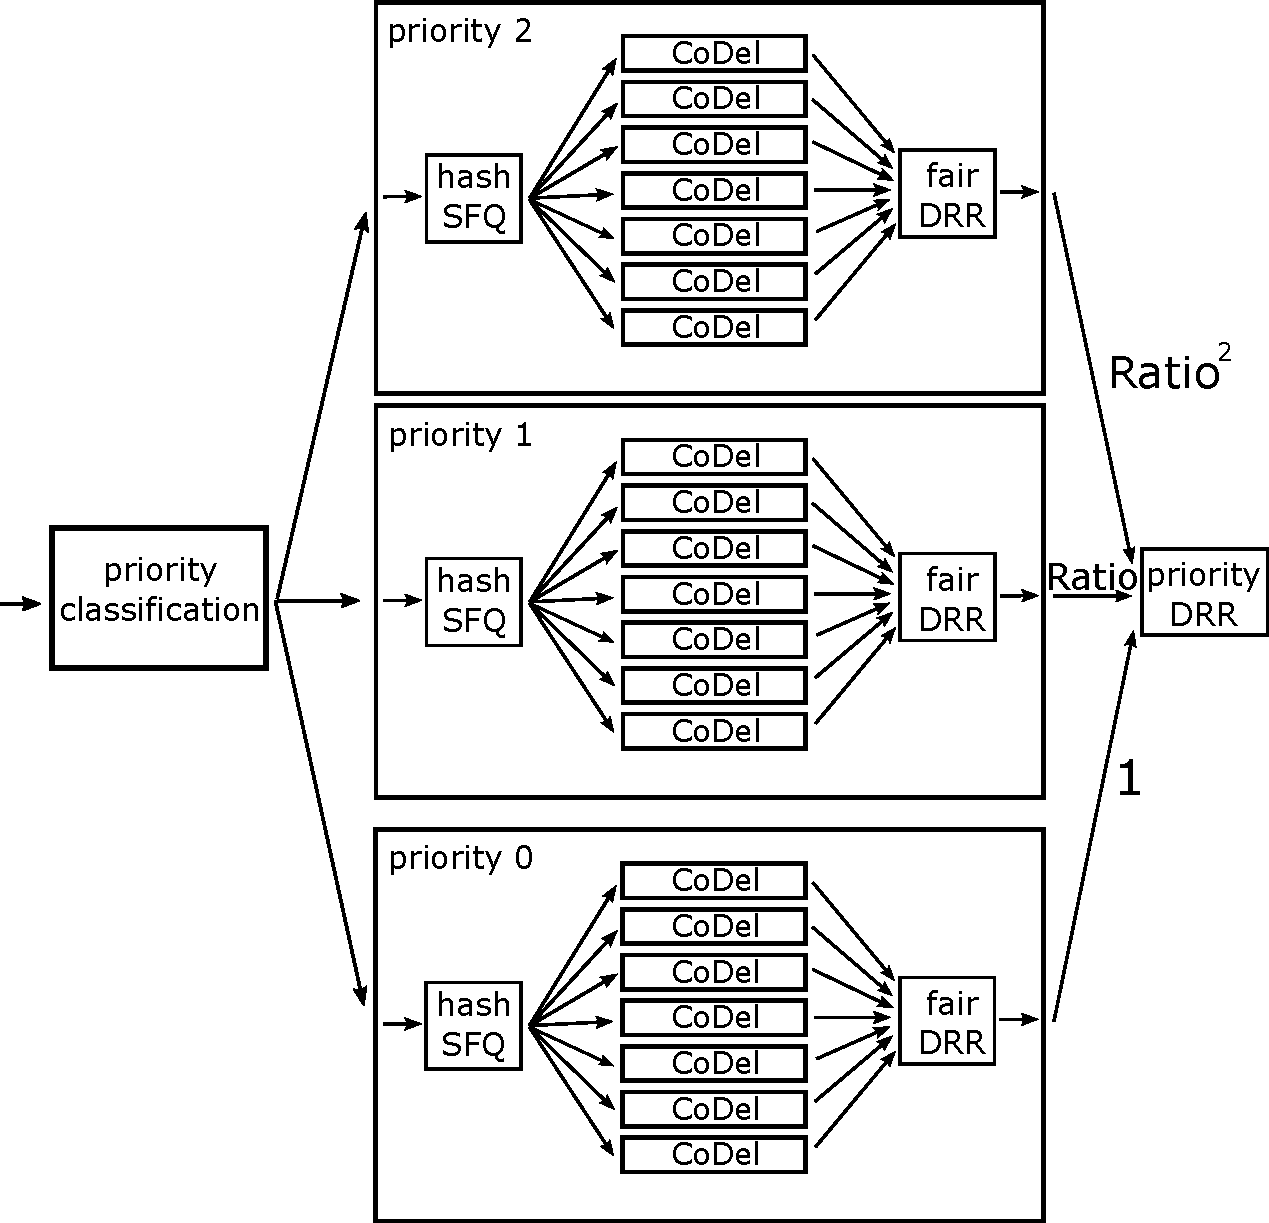
\includegraphics[width=137mm]{drawings/msfc}
	\caption{The MSFC layout}
	\label{fig10:msfc}
\end{figure}

In this thesis, we describe traffic scheduler Multilevel Stochastic Fairness CoDel (MSFC). It combines the ideas of previous work: CoDel and Deficit Round-robin. It uses three-level layout, which is illustrated in Figure \ref{fig10:msfc}. In the highest level, packets are assigned to priority classes. We use non-fair DRR to prioritize more important traffic. Inside the classes, the packets are distributed into flows (based on source and destination IP addresses, ports and protocol) and we use the second, independent fair DRR to schedule traffic within the class. Each flow uses a CoDel algorithm.

It has following parameters:
\begin{itemize}
	\item \X{Prios} --- the number of priority classes.
	\item \X{Flows} --- the number of queues (CoDels) in each priority class (so there are $\X{Prios}*\X{Flows}$ total independent CoDels)
	\item \X{Quantum} --- the quantum parameter of the inner fair DRR (see \autoref{DRR})
	\item \X{Target} --- target delay parameter for CoDel algorithm (see \autoref{CoDel})
	\item \X{Interval} --- Interval parameter for CoDel algorithm (see \autoref{CoDel})
	\item \X{Ratio} --- specifies the ratio of bandwidth of two adjacent priority classes. The ratio is enforced by the outer DRR. MSFC uses \X{Ratio} to compute quantums of all priority classes. The quantums rise exponentially:
	\[
	Q_p = \X{Quantum} \cdot \X{Ratio}^p,
	\]
	where $p$ is the priority of class.
\end{itemize}
For example if there are 3 classes with priorities 0, 1, 2 (like in the Figure \ref{fig10:msfc}), the upstream bandwidth will be distributed in ratio $1:\X{Ratio}:\X{Ratio}^2$.

The ratio of priority class bandwidths is independent of the number of flows in each class. Consider two classes with adjacent priorities 0 and 1. Additionaly, assume that priority 1 class has only one flow backlogged, priority 0 class has 100 flows. The one flow from priority 1 class is guaranteed to receive 2/3 of the bandwidth. The 1/3 is distributed fairly between the remaining 100 flows.

As the Figure \ref{fig10:msfc} shows, enqueue consists of 3 steps. First, MSFC classifies the enqueued packet to determine the priority class. Different implementations may use different classifiers --- i. e. DSCP field of IP header or user-defined criteria. In the second step, MSFC hashes the five-tuple of source address, destination address, source port, destination port and transport protocol. Finally, the packet is timestamped for CoDel and enqueued in the queue determined by the hash.

The dequeue is done in 3 steps as well. First, MSFC uses the outer non-fair DRR to determine the priority class to dequeue a packet. Second, MSFC uses the DRR that runs inside the particular priority class to choose the CoDel queue. Then, MSFC uses the CoDel algorithm (the CoDel dequeue from \autoref{CoDel}), that runs in the queue to dequeue the desired packet.

\section {Implementation}

We have implemented the MSFC algorithm in the Network simulator 3 (ns3) to evaluate its performance in simulated conditions. We also describe existing Linux implementation that can be used for deployment on real hardware.

\subsection {Linux}
\begin{figure}
	\centering
	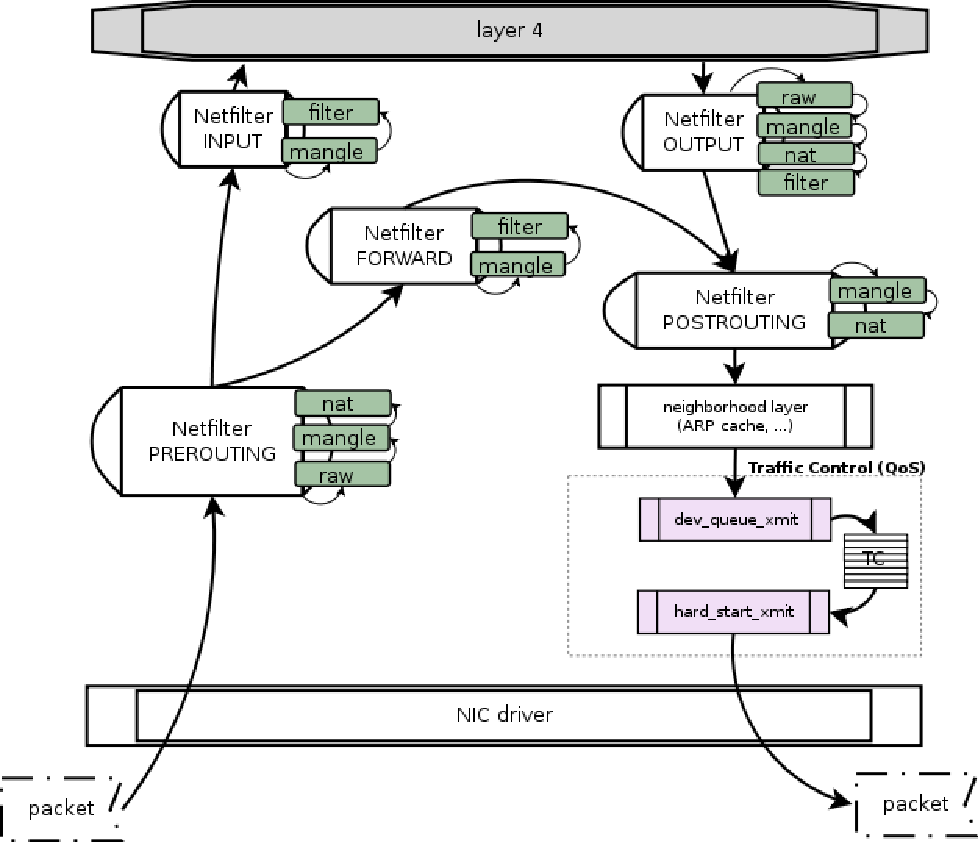
\includegraphics[width=137mm]{drawings/network_stack}
	\caption{Packets traversal through Linux kernel. Picture taken from \cite{linuxCore}}
	\label{fig12:linux}
\end{figure}

To understand the Linux implementation, let us first take a look how Linux controls network traffic. The Figure \ref{fig12:linux} shows the context of traffic control in the Linux kernel. It takes place at the bottom of the third (IP) layer, and stores packets that are ready to be handed over to the link layer (realised by Network Interface Card --- NIC).

There are three kinds of objects used in traffic control: qdisc (queuing discipline), class and filter \cite{tc}. Simply put, qdisc is an abstraction of a traffic scheduler --- its role is to enqueue packets, store them, and choose an outgoing packet when NIC driver asks for one. Every interface must have at least one qdisc --- root qdisc. It may further contain child classes and each class contains exactly one qdisc. Classless qdiscs comprise only one qdisc object. Filter objects allow packet classifying and policing.

When kernel decides a packet is ready to be sent, it enqueues the packet in root qdisc (that exists in every configuration). If the root qdisc is classful, it may end up in any of its child classes. An arbitrary number of filters may be assigned to every class. When a packet arrives to a qdisc with multiple child classes, it calls the filters one by one, until one of them returns with a verdict. The qdisc then enqueues the packet in the child qdisc of the chosen class.

However, the concept of classes and filters is not obligatory to use, it depends on implementation of particular queueing discipline. For example, a classful qdisc may not use any filters to classify a packet, but use a different method instead (e.g. Type of Service field in IP header). Also, a qdisc may be classless in relation to Linux kernel, but still use internal `classes' --- treat different groups of packets differently.

In the kernel, packets are represented by struct \TT{sk\_buff} (socket buffer). This avoids copying of packets and provides attributes like a pointer to the socket where the packet was created, timestamps, length, etc. One of the attributes is (queuing) priority. By default, the kernel sets the priority to the value of the field Type of Service from packet IP header. However, the adminitrator may configure the system to change the priority in postrouting mangle phase (see Figure \ref{fig12:linux}) and thus classify packets before they come to qdisc.

The default qdisc of Linux kernel is \TT{pfifo\_fast}. It is three-band first-come first-serve scheduler. There are 3 independent FIFO queues, one for each priority. \TT{Pfifo\_fast} classifies packets based on priority attribute of \TT{sk\_buff} (it takes 4 least significant bits). The dequeue is simple: it dequeues a packet from the highest priority queue that is not empty.

Every qdisc is connected to the kernel via struct \TT{Qdisc\_ops}. It defines pointers to methods that the kernel calls to operate the qdisc. Every qdisc then defines a variable of type \TT{Qdisc\_ops} and assigns implementations of corresponding methods to the members of the struct. The most important members are:
\begin{itemize}
	\item \TT{enqueue} --- Takes \TT{sk\_buff} argument. It is called every time kernel adds a packet to the qdisc.
	\item \TT{dequeue} --- Returns dequeued packet.
	\item \TT{peek} --- Returns the packet that the qdisc dequeues next.
	\item \TT{init} --- The kernel calls it to initialize the qdisc in the beginning of its operation. Here the qdisc may allocate memory and set its parameters.
	\item \TT{destroy} --- It is called when operation of the qdisc stops. The qdisc should deallocate all its resources (memory, etc.).
	\item \TT{reset} --- The kernel calls it to reset the qdisc into the default (empty) state.
\end{itemize}

The implementation of MSFC follows the 3-level layout of the algorithm. Priority class is represented by struct \TT{msfc\_prioclass} and one CoDel flow by struct \TT{msfc\_flow}. The amount of memory that the implementation needs is constant throughout the lifetime of the qdisc, and it can be computed from parameters \X{Prios} and \X{Flows}. MSFC needs an array of priority classes of size \X{Prios} and an array of CoDel flows of size $\X{Prios} * \X{Flows}$. The implementation allocates all the memory in the initialization (\TT{msfc\_init}) of the qdisc.

The enqueue function needs to determine the right CoDel flow to store the packet. Priority is taken solely from priority attribute of \TT{sk\_buff}. Then, it uses Jenkins hash implemented in Linux to determine the right flow. The packet enqueued is then put in the back of flow using the pointer to the tail in \TT{msfc\_flow}. 

The dequeue implements two DRR algorithms and the CoDel algorithm. For each priority class, the quantums are computed during initialization. The qdisc holds a pointer to the prioclass that is the next as well as its deficit. The \TT{msfc\_prioclass} structs handle the state variables of the inner DRRs, which determine the flow from which the packet is dequeued. Finally, CoDel dequeue is used to obtain the packet --- the \TT{msfc\_flow} struct contains the state of the CoDel algorithm used for the particular flow.

\subsection {ns-3}

Ns-3 (Network Simulator 3) is a discrete-event computer network simulator \cite{ns3}. It provides abstractions of real world objects and devices, and then simulates real (physical) phenomena and technologies as precisely as possible.  It allows us to perform replicable  experiments in a controlled environment that would never be possible in reality.


One of key abstractions of ns-3 is \emph{node}. It represents a network device --- a computer, router, server, etc. Node itself does not have any functionality; It is a container, into which we may install applications, network interfaces and protocols.

\emph{Netdevice} is an abstraction of network interface of a computer. One node may contain more Netdevices, just like a common notebook may contain both Wi-Fi and Ethernet interface cards\todo{je mozny ze oponent uz videl stroj se 600 sitovejma kartama}. Netdevices are closely tied to channels. A channel represents connection between nodes (more specifically two or more Netdevices). For example, it may model something as simple as an Ethernet cable, but also as complex as a three-dimensional space full of obstructions in case of a Wi-Fi channel. The simplest channel is a point-to-point channel, which connects two Netdevices with a configured bandwidth and delay.

\begin{figure}
	\centering
	\includegraphics[width=80mm]{drawings/ns3_internet_stack}
	\captionsetup{justification=centering}
	\caption{Packet traversal through ns3 Internet stack. Picture is based on ns3 documentation \cite[p. 88]{ns3Doc}}
	\label{fig13:ns3}
\end{figure}

The concept of nodes, Netdevices and channels works generally for all networks. To simulate the Internet we must install the Internet stack --- a set of common protocols that are implemented in every device connected to the Internet. That includes TCP, UDP, IP (v4 or v6) or ARP. The whole ns3 stack is displayed in Figure \ref{fig13:ns3}. Traffic control takes place just before the packet is handed over to Netdevice. However, installing traffic control layer to a node is not mandatory; If none is present, ns-3 sends the packets directly to Netdevice.

The ns-3 traffic control simulates the traffic control objects in the Linux kernel. Qdisc is represented by \TT{QueueDisc}, class is \TT{QueueDiscClass} and the filter is named \TT{QueueDiscFilter}. We implemented MSFC as \TT{QueueDisc} and CoDel flow as \TT{QueueDiscClass}. We use filters (one for IPv4 and one for IPv6) to hash packet headers to classify them into the CoDel flows.

\sloppypar
The implementation is as straightforward as possible. We extend the C++ abstract class \TT{QueueDisc}, the most important methods are \TT{DoDequeue} and \TT{DoEnqueue}. We represent the MSFC priority class by C++ class \TT{MsfcPrioClass} and one flow is represented by class \TT{MsfcFlow}. We use the ns-3 implementation of the CoDel algorithm --- there is a CoDel \TT{QueueDisc} assigned to each \TT{MsfcFlow} (using general \TT{QueueDiscClass} mechanism). The actual packets are enqueued in the CoDel \TT{QueueDisc}.

By default, we determine priority of a packet simply by DSCP field in its IP header. However user can change this easily using ns-3 attribute system by providing a different method that classifies packets. 

The usage of ns-3 CoDel has greatly reduced the complexity of implementation --- we only need  to find the right flow during \TT{DoEnqueue} and then enqueue the packet in the \TT{QueueDisc}. First, we determine the enqueuing packet priority to determine the right \TT{MsfcPrioClass}. The priority classes are organised in a structure that maps priorities to corresponding \TT{MsfcPrioClass}. Further, each \TT{MsfcPrioClass} contains a structure, that maps packet hash (computed by assigned filters) to the corresponding \TT{MsfcFlow}. Using the structures, we get the right \TT{MsfcFlow} after which we call the \TT{Enqueue} method of the underlying CoDel \TT{QueueDisc}.

In the dequeue, we implement the two-level DRR. We maintain a list of active priority classes --- the head of the list is the \TT{MsfcPrioClass} that is the next in the outer DRR. Each \TT{MsfcPrioClass} holds its deficit and quantum computed based on the priority when the first packet with the particular priority is enqueued. If the priority class does not have any packets, we deactivate it and remove from the list. We activate it again when a packet of the priority is enqueued.

The same applies to flows within each priority class. Each \TT{MsfcPrioClass} contains a list of active flows and each \TT{MsfcFlow} holds its deficit (we do not need quantum, because it is the same for all the flows). We choose the right flow using the list and the deficit of the flow that is the head of the list, and we dequeue from the underlying CoDel \TT{QueueDisc}.   












